\documentclass[10pt,oneside,slovak,a4paper]{article}

\usepackage[slovak]{babel}
%\usepackage[T1]{fontenc}
\usepackage[IL2]{fontenc} % lepšia sadzba písmena Ľ než v T1
\usepackage[utf8]{inputenc}
\usepackage{graphicx}
\usepackage{url} % príkaz \url na formátovanie URL
\usepackage{hyperref} % odkazy v texte budú aktívne (pri niektorých triedach dokumentov spôsobuje posun textu)
\usepackage{booktabs}
\usepackage{csquotes}

\usepackage{cite}
%\usepackage{times}

\pagestyle{headings}

\title{Učenie sa cudzích jazykov prostredníctvom mobilu\thanks{Semestrálny projekt v predmete Metódy inžinierskej práce, ak. rok 2020/21, vedenie: Fedor Lehocki}} % meno a priezvisko vyučujúceho na cvičeniach

\author{Marko Stahovec\\[2pt]
	{\small Slovenská technická univerzita v Bratislave}\\
	{\small Fakulta informatiky a informačných technológií}\\
	{\small \texttt{xstahovec@stuba.sk}}
	}

\date{\small 15. október 2020}



\begin{document}

\maketitle

\begin{abstract}
Mobilné zariadenia sa postupom času stali neoddeliteľnou súčasťou našich životov a našej spoločnosti ako celku. Od zariadenia, ktoré slúžilo výlučne na telefonovanie a prenos krátkych textových správ, sa vyvinula pomôcka, vďaka ktorej je náš život mnohonásobne jednoduchší a vďaka ktorej sa dá veľa naučiť. Hlavná charakteristika mobile-learningu je ponímaná ako spôsob výučby, ktorý je spontánny, neformálny a všadeprítomný. Síce takýto spôsob výučby nemusí byť práve najefektívnejší, no učiacemu ponúka široké spektrum možností vrátane slobody, času a predovšetkým priestoru, keďže mobilný telefón je použiteľný takmer v akejkoľvek situácii. A preto sa v tejto práci budeme venovať kladom a záporom, t.j. ľahkej dostupnosti, individuálnosti, ale aj nevýhodám malej obrazovky, ukladaniu dát apod. Taktiež sa dotkneme spôsobov, akými by sa dalo také učenie realizovať a taktiež schopnostiam, ktoré sa daným štýlom učenia môžu bohato rozvíjať, napr. gramatika, porozumenie, slovná zásoba apod.
\end{abstract}



\section{Úvod}


Vo svete, v ktorom sa technické zariadenia veľmi rýchlo rozvíjajú, sa bezdrôtová komunikačná technológia nachádza niekde na čele už nezastaviteľného pokroku\cite{Miangah2012}. Každým dňom sa jej pokrytie dostáva hlbšie a hlbľšie do našich životov a učenie sa nie je nijakou výnimkou. Ukázalo sa, že použitie týchto technológií na edukačné účely je v súlade so strategickými vzdelávacími cieľmi, ako je zlepšenie pozornosti a prospechu študentov, podpora diferenciácie učebných potrieb a v neposlednom rade aj oslovovanie študentov, ktorí by inak nemali príležitosť zúčastňovať sa na vzdelávaní\cite{KukulskaHulme2009}. Veľké úsilie sa venovalo aj pochopeniu toho, ako mobilné technológie súvisia s tradičnými aj inovatívnymi spôsobmi výučby a učenia, ukazovaniu použiteľnosti mobilného učenia v širokom spektre aktivít a zdôrazňovaniu najdôležitejších vynárajúcich sa problémov\cite{KukulskaHulme2009}. 

S príchodom internetu všetky možnosti a uplatnenia takéhoto štýlu učenia začali vzrastať exponenciálne, keďže od jednoduchých pracovných listov a učebníc dostupných na internete sa prešlo k praktickým spôsobom, ako je napríklad ponuka audio knihy pri bookovaní dovolenky, ktorá pozostáva z bežnej slovnej zásoby v danom cudzom jazyku podľa danej krajiny. Vzhľadom na mobilné zariadenia konkrétne, tie už do istej miery vďaka svojej všadeprítomnosti ovplyvňujú to, ako sa ľudia učia; na druhej strane je potrebné, aby pedagógovia túto skutočnosť využívali vo svoj prospech\cite{KukulskaHulme2009}. Výhody práve týchto zariadení sú efektívne uplatňované na vedných predmetoch ako sú geografia a biológia, kde sa obsah učiva dá jednoducho graficky spracovať, no podobný prístup sa dá uplatniť aj na cudzie jazyky.

Cieľom tohto článku je zamyslieť sa nad tým, čo mobile-learning ponúka, a znázorniť, v čom tento spôsob výučby vyniká a kde naopak zaostáva. Zameriame sa na výučbu jazykových schopností prostredníctvom mobilného zariadenia (mobile assisted language learning - ďalej len \emph{MALL})\ref{ml}, uvedieme schopnosti, ktoré sa takto primárne rozvíjajú\ref{mall}, kriticky zohľadníme výhody a nevýhody tohto princípu\ref{vyhodyanevyhody} a na záver sa pozrieme aj na jeden konkrétny experimentálny príklad z praxe\ref{experiment}. No predtým, ako sa pozrieme na konkrétne príklady, je dôležité si objasniť, čo sa rozumie pod pojmom "mobile learning".


\section{Mobile learning} \label{ml}

Vysoká popularita mobilných zariadení má za následok okrem zmeny našich životných štýlov aj trendy v učení a komunikácii. No aj napriek tejto všadeprítomnej prezencie zatiaľ neexistuje jednoznačná definícia pre "mobile learning"\cite{Kim2012}. Čiastočne je to preto, lebo táto oblasť podlieha rapídnej evolúcii, a čiastočne pre nejednoznačnosť pojmu "mobile", ktorý môže mať viacero významov\cite{KukulskaHulme2009}. Mobilitu je potrebné chápať nielen z hľadiska priestorového pohybu, ale aj spôsobov, ako môže tento pohyb umožniť posúvanie času a prekračovanie hraníc\cite{KukulskaHulme2009}. Netreba zabúdať na fakt, že technologický progres je ako loď na otvorenom mori, a tak nemožno jasne predpokladať, či používanie mobilného telefónu bude rozšírené v takej podobe, ako je tomu dnes. 

Na druhej strane je možné tvrdiť, že zariadenia, ktoré študenti používajú, nie sú relevantné; dôležitá je predstava mobility a budovanie učebných postupov v tomto procese\cite{KukulskaHulme2009}. El-Hussein a Cronje\cite{Hussein} definovali koncept mobility v troch oblastiach: mobilita technológie, mobilita učenia a mobilita študenta\cite{Kim2012}. 

Mobilitu technológie možno zhrnúť do niekoľkých pojmov, t.j. smartfóny, digitálne kamery, notebooky, GPS zariadenia alebo iné technológie, ktoré sú vybavené bezdrôtovým aplikačným protokolom. Takéto mobilné technológie umožňujú používateľom vykonávať rôzne sociálno-interaktívne činnosti vrátane komunikácie, používania aplikácií, zberu informácií či relaxu\cite{Kim2012}.

Mobilitu učenia definuje niekoľko prívlastkov, ktoré charakterizujú nové možnosti edukačného prístupu: personalizovaný, zameraný na študenta, situovaný, spolupracujúci a všadeprítomný. Študenti majú v takýchto podmienkach osobné a jedinečné skúsenosti v kontexte, v ktorom sa nachádzajú. Pokiaľ ide o vek, miesto, čas alebo trvanie, tak tie nepredstavujú nijaké obmedzenia\cite{Kim2012}. 

A v neposlednom rade kladie mobile learning dôraz na individualitu študentov, ktorým sa podmienky prisposôbujú podľa ich vlastných potrieb. Práve vďaka tomu môže byť ich študijný progres čo najefektívnejší a najproduktívnejší.

Stručne povedané, mobilné učenie upriamuje našu pozornosť na mobilitu, ale aj na jej účinky. Vďaka vhodnej technológii sa môžu študenti prostredníctvom mobilných zariadení vzdelávať a podieľať na činnostaich, ktoré nie sú obmedzované pohybom či inými negatívnymi faktormi.

%Z obr.~\ref{f:rozhod} je všetko jasné. 
%\begin{figure*}[tbh]
%\centering
%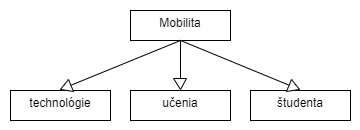
\includegraphics[scale=1.0]{diagram.pdf}
%\caption{Rozhodujúci argument.}
%\label{f:rozhod}
%\end{figure*}

\section{Výhody a nevýhody} \label{vyhodyanevyhody}

Spomedzi všetkých moderných komunikačných zariadení patria mobilné telefóny k jedným z najefektívnejších médií, najmä ak sa pozeráme na pomer prenosnosti a množstvom možností, ktoré poskytujú. Pomocou takéhoto výučbového zariadenia môže študent riadiť svoj vlastný proces učenia vo svojom priestore na základe svojho kognitívneho stavu \cite{Miangah2012}. 

Z týchto faktov vyplýva najväčšia výhoda mobile-learningu - učenie sa v individuálne prispôsobenom prostredí, ktoré môže prebiehať online ale aj offline. Vďaka tomu sa študenti môžu učiť cestou v autobuse, vonku či v práci, počas čakania v rade, alebo na akomkoľvek inom vhodnom mieste. Tento rýchly a flexibilný prístup k materiálom a nástrojom na výučbu jazykov zvyšuje motiváciu a autonómiu študentov v učení sa jazykov \cite{Kim2012}. To podporuje individuálne študijné návyky, ktoré sa môžu prejaviť v rôznych formách aj pri iných typoch štúdia.

Ďalšou nepopierateľnou výhodou je efektívnosť, t.j. možnosť učiť sa formou, ktorá nepôsobí nanútene. Tento aspekt je braný ako výhoda preto, lebo bežný študent nevie podať 100\%-ný výkon v činnosti, ktorá mu je nanútená. Túto psychologickú bariéru každého študenta možno zbúrať mnohými spôsobmi; napríklad mobilnou aplikáciou, v ktorej z rozhádzaných písmen možno skladať slová v cudzom jazyku.

Je dobré spomenúť aj fakt, že množstvo zdrojov, z ktorých sa dá cudzí jazyk naučiť, je prostredníctvom MALL-u takmer neobmedzený vďaka existencii internetu.

Široký vplyv trhu zvýšil popularitu mobilných telefónov, čo vytvorilo možnost pre učiteľov poskytovať nástroje a softvér pre študentov vo vyučovacích kontextoch\cite{Miangah2012}. Okrem toho sú mobilné telefóny v porovnaní s inými bezdrôtovými zariadeniami, ako sú prenosné počítače, pomerne lacné a majú funkciu internetového prehliadača dostupného vo väčšine zariadení\cite{Miangah2012}.

Napriek veľkému množstvu výhod, MALL prináša zopár svojich vlastných nedostatkov, ktoré v sebe tradičný spôsob výučby nezahŕňa. Jedným z najjednoznačnejších nedostatkov je prítomnosť obrazovky mobilného zariadenia, ktorá nielen že je v niektorých situáciách primalá na čítanie, no taktiež je aj veľmi náročná na zrak študenta, čo môže viesť k rôznym zdravotným problémom.

Nemožno zabúdať aj na fakt, že mobilné zariadenia nie sú vyrábané tak, aby slúžili ako učebná pomôcka, a preto je niekedy náročné nájsť vhodný spôsob ako ich v tomto smere využívať. Pri implentácií MALL by sa mal brať do úvahy aj sociálny kontakt, ktorý je značne obmedzený pri používaní mobilného zariadenia.

Ďalšou charakteristickou črtou moderných aplikácií pre štúdium je aj to, že časť z nich nie je zadarmo, čo v prípade kníh poskytnutých školou nemusí platiť. Problémom takýchto aplikácií býva aj to, že podporujú osobné učenie v súkromí, no nepodporujú individuálne prispôsobenú výučbu.





\section{MALL a schopnosti, ktoré obohacuje} \label{mall}

Ako sme už vyššie spomínali, MALL využíva mobilné technológie pohodlným a užitočným spôsobom. Práve tento spôsob je výhodný v tom, že nenúti študentov sedieť v učebni pri kope plnej pracovných listov, ale umožňuje im študovať kedy a kde sa im zachce. A keďže ovládanie angličtiny sa považuje za jeden z hlavných faktorov profesionálneho úspechu a kritérium vzdelávania v mnohých komunitách, poskytovanie pohodlnejšieho prostredia pri výučbe je jedným zo strategických krokov zameraných na zlepšenie výsledkov študentov\cite{Miangah2012}. V nasledujúcich sekciách sa teda povenujeme jazykovým zručnostiam, ktoré MALL primárne rozvíja:

\begin{enumerate}
\item Slovná zásoba~\ref{mall:slovnazasoba}
\item Porozumenie~\ref{mall:porozumenie}
\item Gramatika~\ref{mall:gramatika}
\item Výslovnosť~\ref{mall:vyslovnost}
\end{enumerate}


\subsection{Slovná zásoba} \label{mall:slovnazasoba}

Typ aktivít zameraných na učenie sa slovnej zásoby pomocou mobilného telefónu je nespočetne mnoho. K jedným z najpopulárnejších patria mobilné aplikácie ako napr. Duolingo, ktoré ponúkajú jednoduchý prístup k mnohým jazykom a zobrazujú ich v hravej forme. Stačí si len vybrať jazyk a vypĺňať krížovky či počúvať nahrávky. Posielanie e-mailov alebo SMS študentom je bežný spôsob učenia sa novej slovnej zásoby na základe lekcií absolvovaných na hodine. V štúdii Kennedy a Levy boli študentom posielané správy pokrývajúce známe slová v nových kontextoch prostredníctvom SMS na ich mobilné telefóny deväť alebo desaťkrát týždenne. Výsledky naznačili, že správy boli veľmi užitočné pri učení slovnej zásoby\cite{Kennedy2008}. 

Učenie sa slovnej zásoby môže byť obohatené grafickým prístupom, ktorý sa dá jednoducho zobraziť na mobilných telefónoch študentov. Takýto prístup v kombinácii s riešením úloh a cvičení prostredníctvom mobilnej obrazovky predstavuje veľmi efektívny spôsob ako si upevniť slovnú zásobu.

\subsection{Porozumenie} \label{mall:porozumenie}

\paragraph{Chápanie textu.}
Pod chápanie textu spadá ako sluchové porozumenie, tak aj porozumenie pri čítaní. S aktuálnou generáciou mobilných telefónov je možné navrhnúť multimediálny systém na výučbu posluchových schopností pomocou posluchových cvičení\cite{Miangah2012}. To posúva poslucháča priamo do autentickej konverzácie či monológu, na ktorých si môže prakticky vyskúšať a trénovať chápanie daného jazyka. Ľahko realizovateľnou praktikou v školskom prostredí je taktiež počúvanie textu hlasovou službou na mobilných telefónoch študentov, po ktorom nasleduje kvíz s porozumením posluchu založenom na texte.

Čítanie s porozumením je taktiež jednou z najlepších praktík pre rozvoj jazykových schopností. Čítanie textu v cudzom jazyku má rovnaký efekt ako sluchové porozumenie - posúva čitateľa priamo do autentickej situácie, no čítanie pôsobí na iný zmysel a tým je práve zrak. Práve tento spôsob môže byť použitý v mnohých formách ako napr. nastavenie si mobilného telefónu do cudzieho jazyka či čítanie správ v cudzom jazyku. Takýmto nepriamym učením sa slovná zásoba a chápanie dostávajú prirodzeným a efektívnym spôsobom do povedomia študenta.

\subsection{Gramatika} \label{mall:gramatika}

Pravidlá gramatiky sú taktiež neoddeliteľnou súčasťou akéhokoľvek jazyka. Tieto zručnosti sa dajú podávať viacerými spôsobmi, no učenie sa gramatických pravidiel môže byť prítomnosťou mobilného telefónu jemne povýšené, keďže ide o nie veľmi záživnú aktivitu. Je možné sa ich naučiť prostredníctvom špeciálne navrhnutých mobilných aplikácií, po ktorých môžu nasledovať aktivity s výberom možností \enquote{true/false} alebo aj doplňovanie do medzier \enquote{fill-in the blanks}. 


\subsection{Výslovnosť} \label{mall:vyslovnost}

Druhá generácia mobilných zariadení umožňuje svojim používateľom prístup k multimediálnym funkciám vrátane tých posluchových a hovoriacich\cite{Miangah2012}. Vďaka takýmto zariadeniam si môžu študenti stiahnuť slovníky do PDA1 so zvukovými funkciami, aby sa mohli naučiť správnu výslovnosť neznámych alebo nových slov, aby mohli plniť svoje učebné potreby\cite{Miangah2012}.

Okrem tejto výhody je umožnený aj prenos hlasových správ, vďaka ktorým môžu učitelia odhaliť isté vyslovnostné nedostatky. Takto sa dá vylepšiť nielen výslovnosť, ale aj komunikačné schopnosti študentov prostredníctvom rôznych funkcií systému, ako je napríklad poskytnutie online slovníka na hľadanie neznámych slov a ich správneho fonetického tvaru a podobne\cite{Miangah2012}.



\section{Experiment} \label{experiment}

\paragraph{Experiment zo strednej školy Zaban Amooz v Mahabade\cite{Azar2014}.} Účastníkmi štúdie boli štyri triedy v skupine študentov EFL študujúcich na strednej škole Zaban Amooz. 70 študentov sa zapísalo na konverzačný krúžok, v ktorom sa experiment vykonával. Účastníci boli rozdelení do dvoch rovnomerných skupín a následne absolvovali Oxford Placement Test, aby sa zistilo, ako sú na tom s počúvaním a chápaním anglického jazyka. Rozdiely medzi skupinami boli minimálne, a teda 35 náhodných účastníkov bolo pridelených do experimentálnej skupiny a zvyšných 35 ostalo v porovnávacej skupine.

Učebné postupy používané v obidvoch skupinách boli podobné; obidve skupiny mali hodiny trikrát do týždňa od 17:00 do 19:00 a tieto hodiny trvali celkovo šesť týždňov.

Každá téma, ktorá bola vyučovaná, pozostávala z cvičení venovaných zručnostiam, ktoré boli vysvetlené na začiatku daných hodín. Jediným rozdielom medzi skupinami bolo to, že počas celých šiestich týždňov boli pre experimentálnu skupinu prezentované rôzne audioknihy pre dané témy. Prvých 10 minút bolo venovaných predstaveniu audiokníh, aby ich experimentálna skupina mohla využiť čo najefektívnejšie. Po šiestich týždňoch takéhoto vyučovania absolvovali obe skupiny post-test, aby sa zmerali zlepšenia počúvania s porozumením. Štatistika výsledkov porovnávania priemerných hodnôt oboch skupín po teste je uvedená v tabuľkách nižšie.\\


%\begin{table}[]
%\begin{tabular}{@{}|l|c|c|c|c|@{}}
%\toprule
%Počúvanie s porozumením & N  & Priemer  & Smerodajná odchýlka & Štandardná chyba priemeru \\ \midrule
%Experimentálna skupina  & 35 & 66.31429 & 8.529435            & 0.68                      \\ \midrule
%Porovnávacia skupina    & 35 & 52.88571 & 8.601544            & 1.37                      \\ \bottomrule
%\end{tabular}
%\end{table}


\begin{table}[tbh]
\centering
\begin{tabular}{@{}|l|c|c|c|@{}}
\toprule
Počúvanie s porozumením & N  & Priemer  & Smerodajná odchýlka \\ \midrule
Experimentálna skupina  & 35 & 66.31429 & 8.529435            \\ \midrule
Porovnávacia skupina    & 35 & 52.88571 & 8.601544            \\ \bottomrule
\end{tabular}
\caption{\label{tab:Štatistika}Štatistika pre obe skupiny po post-teste}
\end{table}

Ako ukazuje tabuľka, priemer experimentálnej skupiny bol vyšší ako priemer porovnávacej skupiny, čo znamená, že experimentálna skupina prekonala porovnávaciu skupinu. Smerodajná odchýlka bola tiež nižšia ako tá porovnávacej skupiny; to znamená, že výsledky experimentálnej skupiny boli homogénnejšie.



\section{Záver} \label{zaver} % prípadne iný variant názvu

Cieľom tohto článku bolo predstaviť mobile-learning a jeho uplatnenie pri výučbe jazykov ako techniku, ktorá nemusí úplne nahradiť tradičný spôsob výučby. Tento dokument ukazuje veľký potenciál MALL-u a pripomína, ako rýchlo sa svet mobilných technológií mení, a preto, efektívny dizajn a použitie mobilných zariadení, je potrebné ďalej študovať, keďže koncept MALL-u nevznikol preto, aby sa knihy a učebne prestali používať.

Ak je možné, aby preferencie a potreby študentov boli v ich vlastných rukách, musia mať mobilné technológie pri uskutočňovaní tohto cieľa jasnú úlohu, keďže mobilné zariadenia umožňujú učenie mimo dosahu učiteľa\cite{KukulskaHulme2009}. To je možné vnímať ako hrozbu, a preto je nevyhnutné, aby sa vyvinuli návrhy, ktoré by určili, čo sa najlepšie učí v triede a čo by sa malo učiť mimo študentských učební a ako zosúladiť tieto dva svety do jedného celku.

%\acknowledgement{Ak niekomu chcete poďakovať}


% týmto sa generuje zoznam literatúry z obsahu súboru literatura.bib
\bibliography{literatura}
\bibliographystyle{plain} % prípadne alpha, abbrv alebo hociktorý iný
\end{document}
